%%%%%%%%%%%%%%%%%%%%%%%%%%%%%%%%%%%%%%%%%%%%%%%%%%%%%%%%%%%%
%%% Neural Computation Manuscript
%%% Virtual Zebrafish: Active Inference in a Spiking Neural
%%% Network Model of the Larval Zebrafish Brain
%%%%%%%%%%%%%%%%%%%%%%%%%%%%%%%%%%%%%%%%%%%%%%%%%%%%%%%%%%%%
\documentclass[12pt]{article}

% --- Page layout (Neural Computation: single column, double-spaced) ---
\usepackage[margin=1in]{geometry}
\usepackage{setspace}
\doublespacing

% --- Mathematics ---
\usepackage{amsmath,amssymb,amsfonts}

% --- Graphics ---
\usepackage{graphicx}
\usepackage{float}

% --- Tables ---
\usepackage{booktabs}
\usepackage{multirow}

% --- Bibliography (APA style via natbib) ---
\usepackage{natbib}
\bibliographystyle{apalike}

% --- Cross-references and hyperlinks ---
\usepackage{hyperref}
\hypersetup{colorlinks=true, linkcolor=blue, citecolor=blue, urlcolor=blue}

% --- Miscellaneous ---
\usepackage{enumitem}
\usepackage{xcolor}

% =====================================================================
\title{A Biologically Grounded Virtual Zebrafish: Active Inference and
Predictive Coding in a Developmental Spiking Neural Network}

\author{Anonymous}

\date{}

\begin{document}
\maketitle

% =====================================================================
\begin{abstract}
We present a spiking neural network (SNN) model of the larval zebrafish
brain that implements a complete perception--action loop under the
active inference framework.
The model is constructed through a 42-step developmental curriculum,
each step adding a biologically motivated computational module---from
binocular retinal sampling and tectal processing through predictive
coding, neuromodulation, and goal-directed planning to emotional
regulation and interoceptive awareness.
The neural architecture features two-compartment predictive coding
neurons with apical feedback and goal-driven attention, a dopamine
system implementing temporal-difference reward prediction error,
an amygdala fear circuit, allostatic interoception, hippocampal
place cells, and a VAE-based world model---all coordinated by
Expected Free Energy (EFE) minimization over four goal
states (forage, flee, explore, social).
Motor output is generated through a spinal central pattern generator
with biologically realistic bout dynamics, Mauthner cell escape
reflexes, and prey capture kinematics.
The system achieves 84/100 on a decision rationality benchmark
comprising five structured cognitive scenarios, demonstrates online
reinforcement learning that doubles food intake over 20 episodes,
and maintains energy homeostasis with adaptive foraging under
predator threat.
All learning uses biologically plausible local rules---genomic
pretraining, RPE-gated Hebbian plasticity, PE-driven anti-Hebbian
feedback learning, and TD-based EFE weight adaptation---without
backpropagation through time.
The model demonstrates that the free energy principle provides a
unified computational framework for perception, action, learning,
and homeostatic regulation within a single virtual organism.

\medskip
\noindent\textbf{Keywords:} active inference, predictive coding,
spiking neural network, zebrafish, free energy principle,
neuromodulation, reinforcement learning, virtual organism
\end{abstract}

% =====================================================================
\section{Introduction}\label{sec:intro}

Understanding how vertebrate brains generate adaptive behavior from
neural circuits remains a central challenge in computational
neuroscience.
While substantial progress has been made in characterizing individual
brain regions and their functions, a critical gap persists between
abstract computational models of cognition and biologically realistic
neural simulations.
Abstract models of active inference \citep{friston2010,parr2022}
and predictive coding \citep{rao1999,bogacz2017} provide elegant
normative accounts of brain function but are typically formulated at
a level of abstraction far removed from specific neural circuits.
Conversely, detailed biophysical models of spiking neurons capture
cellular-level dynamics but rarely scale to the complete sensorimotor
loops that generate behavior.

The larval zebrafish (\textit{Danio rerio}, 5--7 days
post-fertilization) offers an ideal model system for bridging this
gap.
Its brain contains approximately 100,000 neurons---small enough for
whole-brain calcium imaging at cellular resolution
\citep{ahrens2013}---yet generates a rich behavioral repertoire
including visually guided prey capture \citep{bianco2015}, predator
avoidance with Mauthner cell escape reflexes \citep{temizer2015,dunn2016},
social behavior and shoaling \citep{dreosti2015}, and optomotor
responses \citep{portugues2014}.
The transparency of the larval brain enables simultaneous recording of
neural activity across all major brain regions during behavior, providing
uniquely comprehensive datasets for constraining computational models.
Furthermore, the zebrafish brain contains homologs of all major
vertebrate structures---optic tectum (superior colliculus), pallium
(cortex), habenula, basal ganglia, hypothalamus, and cerebellum---making
it a tractable proxy for understanding general principles of vertebrate
brain organization.

The active inference framework \citep{friston2010,friston2017,parr2022}
proposes that all brain function can be understood as minimizing
variational free energy---an upper bound on sensory surprise.
Under this framework, perception corresponds to updating internal
beliefs to minimize prediction errors (perceptual inference), action
corresponds to changing sensory inputs to match predictions (active
inference), and learning corresponds to optimizing the generative model
parameters (perceptual learning).
Goal-directed behavior emerges from minimizing \emph{expected} free
energy (EFE), which naturally balances pragmatic value (achieving
preferred outcomes) with epistemic value (reducing uncertainty).
This framework provides a principled account of how organisms
simultaneously perceive, act, learn, and plan within a single
information-theoretic objective.

In this paper, we present a computational model---the Virtual
Zebrafish---that implements the active inference framework in a
spiking neural network architecture inspired by the larval zebrafish
brain.
The model is constructed through a 42-step developmental curriculum,
where each step introduces a new computational module corresponding
to a biological brain structure or function.
This developmental approach mirrors biological maturation, where neural
circuits come online progressively, and enables systematic testing at
each stage of complexity.

The key contributions of this work are:
\begin{enumerate}[nosep]
  \item A complete spiking neural network architecture with
    two-compartment predictive coding neurons, goal-driven attention,
    and homeostatic gain control that implements hierarchical free
    energy minimization.
  \item Integration of active inference goal selection, reinforcement
    learning, and Hebbian plasticity within a single sensorimotor loop,
    demonstrating their complementary roles in generating adaptive
    behavior.
  \item A 42-step developmental curriculum that systematically builds
    a virtual organism from retinal sampling to emotional awareness,
    with quantitative evaluation at each stage.
  \item Demonstration that the free energy principle provides a unified
    computational language for exteroceptive perception, interoceptive
    regulation, neuromodulation, and motor control.
\end{enumerate}

The model achieves 84/100 on a decision rationality benchmark,
demonstrates online learning that doubles foraging efficiency, and
maintains adaptive behavior under concurrent predator threat and
energy depletion---all using exclusively local, biologically
plausible learning rules.

% =====================================================================
\section{Related Work}\label{sec:related}

\subsection{Zebrafish Neuroscience}

Whole-brain calcium imaging in larval zebrafish
\citep{ahrens2013} revealed that visuomotor behavior engages
distributed neural networks spanning the optic tectum, hindbrain,
and cerebellum.
\citet{portugues2014} mapped stereotyped activity patterns during
optomotor responses, identifying distinct functional modules for
sensory processing, motor planning, and action execution.
Prey capture in larval zebrafish involves a characteristic sequence
of J-turns, approach swims, and capture strikes, with tectal neurons
encoding prey position in a retinotopic map
\citep{bianco2015}.
Predator avoidance relies on looming-sensitive neurons in the tectum
that trigger Mauthner cell-mediated C-start escape reflexes when the
angular expansion rate of an approaching object exceeds a threshold
\citep{temizer2015,dunn2016}.
Social behavior emerges early in development, with larval zebrafish
showing attraction to conspecifics and modulation of activity by
social context \citep{dreosti2015}.
The habenula plays a critical role in behavioral flexibility, encoding
aversive expectation values that enable adaptive avoidance strategies
\citep{amo2014,jesuthasan2012}.

\subsection{Active Inference and Predictive Coding}

The free energy principle \citep{friston2010} proposes that biological
systems minimize variational free energy---the divergence between their
internal generative model and sensory observations.
Predictive coding \citep{rao1999} implements this minimization through
a hierarchy of prediction errors, where each cortical layer predicts
the activity of the layer below and updates its representation based
on the mismatch.
\citet{bogacz2017} provided a tutorial unification of predictive coding
with Bayesian inference, showing that prediction error minimization
approximates exact Bayesian updating under Gaussian assumptions.
\citet{clark2013} extended this framework to an encompassing theory
of brain function where prediction pervades all levels of neural
processing.
Active inference \citep{friston2017,parr2022} generalizes predictive
coding to action: organisms act to fulfill their generative model's
predictions, selecting policies that minimize expected free energy.
The EFE objective naturally decomposes into pragmatic (reward-seeking)
and epistemic (uncertainty-reducing) components, providing a normative
account of exploration-exploitation trade-offs.
Attention has been formalized as precision optimization---the brain's
allocation of gain to sensory channels in proportion to their expected
reliability and task-relevance \citep{feldman2010}.
Interoceptive inference extends the framework to homeostatic regulation:
organisms minimize prediction errors across both exteroceptive and
interoceptive Markov blankets \citep{seth2016,barrett2015,pezzulo2015}.

\subsection{Spiking Neural Networks and Virtual Organisms}

Biologically detailed spiking neural networks have been used to model
specific neural circuits, with Spaun \citep{eliasmith2012} being a
notable large-scale example that demonstrates cognitive tasks using
2.5 million leaky integrate-and-fire neurons.
However, Spaun focuses on cortical function in primates rather than
whole-organism behavior.
The OpenWorm project \citep{openworm2014} aims to simulate
\textit{C.\ elegans} at cellular resolution but has not yet achieved
complete behavioral repertoires.
\citet{merel2019} developed virtual rodent models using deep
reinforcement learning to control articulated bodies, demonstrating
realistic locomotion but without biological neural architectures.
Animat approaches \citep{wilson1991} pioneered the idea of simulated
organisms but typically used simplified neural networks without
biological grounding.

\subsection{Reinforcement Learning and Dopamine}

The correspondence between temporal-difference (TD) learning
\citep{sutton2018} and dopamine neuron firing patterns
\citep{schultz1997} established a foundational link between
computational reinforcement learning and neurobiology.
Actor-critic architectures map naturally onto basal ganglia circuits,
with the ventral striatum encoding state values and the dorsal
striatum implementing action selection \citep{oquist2004}.
\citet{dabney2020} demonstrated that distributional reinforcement
learning provides a better account of dopamine neuron diversity than
scalar TD error.
The integration of model-free RL (habitual behavior) with model-based
planning (goal-directed behavior) has been extensively studied
\citep{daw2011}, with evidence that these systems compete and
cooperate depending on uncertainty and computational cost.

\subsection{Gap in the Literature}

Despite significant advances in each of these areas, no existing model
combines a spiking neural network architecture with full active
inference (perception, action, learning, and planning), a complete
sensorimotor loop (from retina to motor output), emotional and
interoceptive regulation, and multiple learning systems (genomic,
Hebbian, reinforcement) within a single virtual organism operating
in a complex ecological environment.
The present work addresses this gap by building a comprehensive virtual
zebrafish through a systematic developmental curriculum.

% =====================================================================
\section{Methods}\label{sec:methods}

The virtual zebrafish brain is constructed through 42 developmental
steps, organized here by functional subsystem.
Table~\ref{tab:steps} provides a complete listing of all steps with
their corresponding modules and key equations.

\subsection{SNN Architecture}\label{sec:snn}

\subsubsection{Two-Compartment Predictive Coding Neuron}

Each trainable layer uses a two-compartment neuron model with distinct
somatic and apical dendritic compartments.
The soma integrates bottom-up feedforward input, bounded apical
contribution, and attention bias:
\begin{equation}\label{eq:soma}
  \mathbf{v}_s(t) = \tau_s\,\mathbf{v}_s(t{-}1)
    + (1 - \tau_s)\bigl(\mathbf{x}\,\mathbf{W}_\text{FF}\bigr)
    + f_a\!\bigl(\mathbf{v}_a(t{-}1)\bigr)
    + \alpha_\text{att}\,\mathbf{m}(t),
\end{equation}
where $\tau_s = 0.8$ and the bounded apical coupling is
$f_a(x) = \frac{1}{2}(\sigma(x) - \frac{1}{2})$, constraining
the top-down influence to $[-0.25, +0.25]$.

The apical dendrite receives top-down feedback from the next higher
layer with a one-step delay:
\begin{equation}\label{eq:apical}
  \mathbf{v}_a(t) = \tau_a\,\mathbf{v}_a(t{-}1)
    + (1 - \tau_a)\bigl(\mathbf{h}^{(l+1)}\,\mathbf{W}_\text{FB}\bigr),
  \quad \tau_a = 0.65.
\end{equation}

The prediction error at each layer is the apical--somatic mismatch:
\begin{equation}\label{eq:pred_error}
  \boldsymbol{\varepsilon}^{(l)} = \mathbf{v}_a^{(l)} - \mathbf{v}_s^{(l)}.
\end{equation}

The processing pipeline follows a hierarchical path:
\begin{equation}\label{eq:pipeline}
  \underbrace{\text{Retina}}_{800 \times 2}
  \xrightarrow{\text{topographic}}
  \underbrace{\text{OT}_{L/R}}_{600 \times 2}
  \xrightarrow{\text{lateral inh.}}
  \underbrace{\text{OT}_F}_{800}
  \xrightarrow{}
  \underbrace{\text{PT}}_{400}
  \rightarrow
  \underbrace{\text{PC}_{per}}_{120}
  \xrightarrow{}
  \underbrace{\text{PC}_{int}}_{30}
  \rightarrow
  \begin{cases}
    \text{Motor} & (200) \\
    \text{Eye}   & (100) \\
    \text{DA}    & (50)
  \end{cases}
\end{equation}

Top-down feedback connections form a descending chain:
$\text{DA} \to \text{PC}_\text{int} \to \text{PC}_\text{per}
\to \text{PT} \to \text{OT}_F$.
The frozen topographic layers $\text{OT}_L / \text{OT}_R$ retain
single-compartment dynamics without feedback.

\subsubsection{Goal-Driven Attention Modulator}

Eight attention neurons (two per goal) with slow neuromodulatory
dynamics ($\tau_\text{att} = 0.93$, half-life $\approx 14$ steps)
map the goal probability vector to per-neuron excitability biases:
\begin{equation}\label{eq:attention}
  \mathbf{m}(t) = \tau_\text{att}\,\mathbf{m}(t{-}1)
    + (1 - \tau_\text{att})\bigl(\mathbf{g}\,\mathbf{W}_\text{att}\bigr).
\end{equation}
Each trainable layer receives an additive somatic bias via a learned
projection $\text{att}^{(l)} = \mathbf{m}\,\mathbf{W}_\text{proj}^{(l)}$.
Under the Bayesian brain hypothesis, this implements precision
optimization: the brain allocates computational gain to sensory
channels in proportion to their task-relevance
\citep{feldman2010}.

\subsubsection{Homeostatic Gain Control}

Divisive normalization prevents unbounded activity growth:
\begin{equation}\label{eq:gain_control}
  \mathbf{v}_s \leftarrow
  \begin{cases}
    \mathbf{v}_s \cdot v^*/\text{RMS}(\mathbf{v}_s)
      & \text{if } \text{RMS}(\mathbf{v}_s) > v^*, \\
    \mathbf{v}_s & \text{otherwise},
  \end{cases}
\end{equation}
where $v^* = 5.0$ is the target RMS.
Bidirectional scaling also boosts underactive layers (up to $3\times$),
implementing synaptic scaling \citep{turrigiano2004,turrigiano2008}.

\subsubsection{Free Energy}

The hierarchical free energy aggregates precision-weighted prediction
errors across all layers:
\begin{equation}\label{eq:free_energy}
  F = \sum_{l} \tfrac{1}{2}\,\bar{\pi}_l\,
      \bigl\|\boldsymbol{\varepsilon}^{(l)}\bigr\|^2.
\end{equation}
Precision $\pi_l = \sigma(\gamma_l)$ is adapted via empirical Bayes:
\begin{equation}\label{eq:precision}
  \Delta\gamma = \alpha_\pi\,(|\varepsilon| - \beta)
    - 0.05\,\nu\,\mathbb{1}[\nu > 0.03],
\end{equation}
where $\beta = 0.1$ is the target error level and $\nu$ is the
novelty signal (Bayesian surprise).

\subsection{Sensory Processing}\label{sec:sensory}

\subsubsection{Binocular Retinal Sampling}

Each eye samples a $20 \times 20$ angular grid (400 pixels) with
$\pm 80^\circ$ horizontal and $\pm 20^\circ$ vertical field of view.
Each pixel carries an intensity channel with Gaussian foveation
($G(\alpha) = \exp(-\alpha^2 / 2\sigma^2)$, $\sigma = 12^\circ$)
and a type channel encoding entity identity (food$\,{=}\,1.0$,
obstacle$\,{=}\,0.75$, enemy$\,{=}\,0.5$, colleague$\,{=}\,0.25$,
boundary$\,{=}\,0.12$).
Depth-shaded intensity attenuates exponentially with distance:
$I_\text{depth}(r) = I_\text{raw}(r) \cdot \exp(-d(r)/80)$.

\subsubsection{Lateral Line Mechanosensation}

Sixteen virtual neuromasts (8 per side) detect hydrodynamic flow from
nearby moving entities using a dipole flow model.
Reafference cancellation subtracts predicted self-motion flow via
cerebellar efference copy.
The rear wake signal detects predator approach from behind the
visual field \citep{stewart2013}.

\subsubsection{Olfactory System}

Bilateral nostrils sample two chemical channels: food odor
(Gaussian diffusion from each food item, radius 200\,px) and
alarm substance (Schreckstoff) released by injured or fleeing
conspecifics.
Food odor provides gradient-based chemotaxis beyond the visual field;
alarm substance triggers group flight responses
\citep{jesuthasan2012}.

\subsubsection{Color Vision and Vestibular System}

Four cone channels (UV 360\,nm, blue 415\,nm, green 480\,nm,
red 570\,nm) with color-opponent processing provide entity
disambiguation beyond shape cues.
Otolith-based gravity sensing provides body orientation with a
vestibulo-ocular reflex compensating eye position for head turns.

\subsection{Motor Control}\label{sec:motor}

\subsubsection{Spiking Spinal Central Pattern Generator}

A 32-neuron half-centre oscillator contains 8 V2a excitatory
interneurons, 4 V0d commissural inhibitory neurons, and 4 motor
neurons per side, implemented as leaky integrate-and-fire units:
\begin{equation}\label{eq:cpg}
  v_i(t{+}1) = \tau_m\,v_i(t) + (1-\tau_m)(I_\text{ext}
    + I_\text{syn} + \xi),
\end{equation}
where $I_\text{syn} = w_\text{exc}\,\bar{s}_\text{exc}
- w_\text{inh}\,\bar{s}_\text{contra}$ produces alternating
left/right bursts.
Descending drive from the brain modulates burst frequency.

\subsubsection{Motor Primitive Repertoire}

The brain provides directional intent; the motor system controls
bout timing through burst (3--5 steps, full speed), glide (2 steps,
decaying speed), and idle phases with goal-modulated inter-bout
intervals (flee: 1 step, forage: 2, explore: 3)
\citep{marques2018}.

\subsubsection{Mauthner Cell C-Start Escape Reflex}

A looming detector computes the $\ell/v$ ratio (angular size /
expansion rate).
When $\ell/v < 10$ and enemy pixels exceed 3, a stereotyped C-start
fires: 1.5\,rad C-bend (2 steps) followed by a $1.6\times$
propulsive stroke (2 steps), with a 12-step refractory period
\citep{temizer2015}.

\subsubsection{Prey Capture Kinematics}

A finite state machine implements three-phase prey capture:
J-turn (3 steps, slow precise orientation), approach swim
(5 steps, half speed), and strike (2 steps, $1.4\times$ burst
with enlarged eat radius) \citep{bianco2015}.

\subsubsection{Cerebellum Forward Model}

A Marr-Albus-Ito architecture with granule cell sparse expansion
($4\times$, 50\% active) and Purkinje cell linear readout predicts
6 sensory consequences of motor commands.
Climbing fiber error drives LTD at parallel fiber--Purkinje synapses,
providing motor correction and reafference predictions.

\subsection{Decision Making}\label{sec:decision}

\subsubsection{Expected Free Energy}

Four discrete goals $\mathcal{G} = \{\text{FORAGE}, \text{FLEE},
\text{EXPLORE}, \text{SOCIAL}\}$ are scored by expected free energy:
\begin{equation}\label{eq:efe}
\begin{aligned}
  G_\text{FORAGE} &= 0.2\,\mathcal{U} - 0.8\,p_\text{food}
    + 0.2\,(0.5 - \text{DA}) + 0.15
    - 0.6\,s^* + 0.15\,p_\text{enemy}, \\
  G_\text{FLEE} &= 0.1\,\text{CMS} - 0.8\,p_\text{enemy} + 0.20
    + 0.4\,s^*, \\
  G_\text{EXPLORE} &= 0.3\,\mathcal{U}
    - 0.5\,(p_\emptyset + p_\text{env})
    + 0.1\,\text{CMS} + 0.20 + 0.2\,s^*, \\
  G_\text{SOCIAL} &= 0.2\,\mathcal{U}
    - 0.6\,p_\text{colleague}
    + 0.15\,p_\text{enemy} + 0.25 + 0.15\,s^*,
\end{aligned}
\end{equation}
where $\mathcal{U} = 1 - \frac{1}{2}(\pi_\text{OT} + \pi_\text{PC})$
is model uncertainty, $s^*$ is starvation risk, and lower EFE
indicates a more preferred goal.

The policy posterior uses a softmax with inverse temperature
$\beta = 2.0$:
\begin{equation}\label{eq:posterior}
  \pi(g_i) = \frac{\exp(-\beta\,(G_i - G_\text{min}))}
                   {\sum_j \exp(-\beta\,(G_j - G_\text{min}))}.
\end{equation}

\subsubsection{Bayesian Survival Trade-off}

Starvation risk modulates all four goal EFE values:
\begin{equation}\label{eq:starvation}
  s = \max\!\bigl(0, (0.5 - e)/0.5\bigr),
  \quad s^* = \begin{cases} s^{0.5} & \text{if } e < 0.3, \\ s & \text{otherwise}, \end{cases}
\end{equation}
where $e$ is the energy ratio.
When both predator threat and starvation are active, the system
performs Bayesian model comparison via the EFE softmax rather than
hard-coding a flee override, consistent with state-dependent risk
sensitivity in zebrafish \citep{lima1990}.

\subsubsection{Habenula: Behavioral Flexibility}

The habenula computes a frustration signal from accumulated negative
RPE per goal.
When frustration exceeds a threshold, a strategy switch is forced,
implementing learned helplessness and behavioral flexibility
\citep{amo2014}.

\subsection{World Models}\label{sec:world_models}

\subsubsection{VAE World Model}

A variational autoencoder learns a 16-dimensional latent belief state
$\mathbf{z}$ from pooled tectal output concatenated with a
multi-modal state context.
The encoder implements amortized variational inference
\citep{kingma2014}:
\begin{equation}\label{eq:vae}
  q_\phi(\mathbf{z}|\mathbf{o}) = \mathcal{N}(\boldsymbol{\mu}_\phi,
    \text{diag}(\boldsymbol{\sigma}_\phi^2)),
\end{equation}
trained by maximizing the ELBO (minimizing variational free energy):
\begin{equation}\label{eq:elbo}
  \mathcal{L}_\text{VAE} =
    \underbrace{\text{MSE}(\hat{\mathbf{o}}, \mathbf{o})}_{\text{accuracy}}
    + \underbrace{0.1\,D_\text{KL}(q(\mathbf{z}|\mathbf{o})\,\|\,p(\mathbf{z}))}_{\text{complexity}}.
\end{equation}

A transition model predicts next-step latent states:
$\mathbf{z}_{t+1} = \mathbf{z}_t + 0.3\,\tanh(f_\text{trans}([\mathbf{z}_t \| \mathbf{a}_t]))$.
Planning simulates 3-step trajectories per goal through the transition
model, scoring via pragmatic (utility) and epistemic (information gain)
terms \citep{friston2017}.

\subsubsection{Geographic Model}

A $40 \times 30$ grid maintains obstacle occupancy, food density,
and epistemic value layers, updated from retinal observations.
This provides spatial knowledge that persists across episodes,
analogous to hippocampal allocentric maps in zebrafish dorsolateral
pallium \citep{broglio2015}.

\subsubsection{Predator Model}

A Kalman filter maintains beliefs over predator state
$\mathbf{s} = [x, y, v_x, v_y, \text{intent}]$ with object
permanence: when the predator leaves the visual field, beliefs
propagate forward with growing uncertainty rather than dropping
to zero.
Hunting intent is inferred from velocity direction toward the fish.

\subsubsection{Internal State Model}

A metabolic cost model maintains learned drain and gain rates per
behavioral mode, enabling counterfactual policy comparison: for each
goal, a 30-step energy trajectory is simulated to estimate energy
risk and time-to-starvation.
This implements counterfactual active inference---evaluating
futures before committing to a policy \citep{seth2016,craig2009}.

\subsection{Neuromodulation}\label{sec:neuromod}

\subsubsection{Dopamine System}

TD-style reward learning computes reward prediction error:
\begin{equation}\label{eq:dopamine}
  \text{RPE}(t) = r(t) - V(t), \quad
  V(t{+}1) = (V(t) + \alpha_V\,\text{RPE}(t)) \cdot \delta_V,
\end{equation}
with $\alpha_V = 0.05$, $\delta_V = 0.98$.
The dopamine level $\text{DA}(t) = \sigma(\beta_\text{DA} \cdot
\text{RPE}(t)) + \xi$, clamped to $[0,1]$, modulates basal ganglia
leak rate, thalamic gain, and precision sensitivity
\citep{schultz1997}.

\subsubsection{Amygdala Fear Circuit}

A persistent threat arousal signal $\alpha \in [0,1]$ integrates
retinal enemy detection, predator proximity, and allostatic stress
with asymmetric dynamics (fast rise 60\%, slow decay 15\% per step):
\begin{equation}\label{eq:amygdala}
  \alpha(t) = \begin{cases}
    0.4\,\alpha(t{-}1) + 0.6\,r_\text{raw} & r_\text{raw} > \alpha(t{-}1), \\
    0.85\,\alpha(t{-}1) & \text{otherwise}.
  \end{cases}
\end{equation}
Downstream effects include classification boost
($p_\text{enemy} \mathrel{+}= 0.3\alpha$), stress feedback, and
flee burst scaling.

\subsubsection{Allostatic Interoception}

Three interoceptive variables---hunger $h$, fatigue $f$, and
stress $\sigma$---are tracked by predictive models generating
interoceptive prediction errors $\varepsilon_x^\text{intero}
= \hat{x} - x^*$ relative to homeostatic setpoints
\citep{seth2016,barrett2015}.
These errors bias EFE priors: hunger PE promotes foraging, stress PE
promotes fleeing, and fatigue PE promotes resting \citep{pezzulo2015}.
Precision is modulated under allostatic pressure:
\begin{equation}\label{eq:allo_precision}
  \sigma_E = \frac{\sigma_{E,0}}{1 + 3\,\max(0, h - 0.5)},
  \quad
  \sigma_S = \frac{\sigma_{S,0}}{1 + 2\,\sigma_\text{stress}},
\end{equation}
making the agent increasingly sensitive to survival-relevant signals
under stress \citep{stephan2016}.

\subsubsection{Insula: Interoceptive Awareness}

The insula integrates heart rate, arousal, and emotional valence,
providing a meta-level awareness of the organism's internal state
that modulates goal selection and behavioral urgency.

\subsection{Learning}\label{sec:learning}

\subsubsection{Genomic Pretraining}

Supervised training mimics evolutionary pre-wiring of the motor
pathway using diverse goal contexts (70\% FORAGE, 20\% FLEE,
10\% EXPLORE):
\begin{equation}\label{eq:genomic}
  \mathcal{L} = \|\hat{\tau} - s\,\tanh(2\alpha)\|^2
    + 0.3\,\|\hat{\phi} - s\,\alpha/\pi\|^2,
\end{equation}
where $s = +1$ for approach (food) and $s = -1$ for avoidance (enemy).

\subsubsection{Hebbian Fine-tuning}

RPE-gated Hebbian plasticity refines feedforward connections:
\begin{equation}\label{eq:hebbian}
  \Delta\mathbf{W}_\text{FF} = \eta\,\text{RPE}\,\text{DA}\;
    (\mathbf{x}_\text{pre}^\top \mathbf{x}_\text{post}),
  \quad \eta = 0.0005.
\end{equation}

\subsubsection{PE-Driven Feedback Learning}

Feedback weights are updated by an anti-Hebbian rule derived from
the free energy gradient:
\begin{equation}\label{eq:feedback}
  \Delta\mathbf{W}_\text{FB}^{(l)} =
    -\eta_\text{fb}\;\bigl(\mathbf{h}^{(l+1)}\bigr)^\top
    \boldsymbol{\varepsilon}^{(l)},
  \quad \eta_\text{fb} = 2 \times 10^{-4}.
\end{equation}
This reward-independent rule implements perceptual learning of the
generative model \citep{rao1999,bogacz2017}, distinct from the
reward-modulated feedforward Hebbian rule.
The feedforward path is frozen during dedicated feedback training
phases to prevent representational drift.

\subsubsection{Object Classification}

A two-layer classifier ($804 \to 128 \to 5$) is trained on bilateral
retinal type channels augmented with aggregate pixel-count features:
\begin{equation}\label{eq:classifier}
  \mathbf{x}_\text{cls} = [\mathbf{t}_L \| \mathbf{t}_R \|
    \tilde{n}_\text{obs}\;\tilde{n}_\text{ene}\;
    \tilde{n}_\text{food}\;\tilde{n}_\text{bnd}],
\end{equation}
where $\tilde{n}_k = n_k/50$ are normalized pixel counts.
This achieves 100\% validation accuracy across all five classes.

\subsubsection{Online RL Critic}

A TD learning critic $V_\phi: \mathbb{R}^{16} \to \mathbb{R}$
adapts EFE weights online:
\begin{equation}\label{eq:td}
  y_t = r_t + (1-d_t)\,\gamma\,V_\phi(s_{t+1}), \quad \gamma = 0.95.
\end{equation}
TD error modulates EFE weights per goal:
$\Delta w_g = \eta_\text{EFE}\,\delta\,\pi(g)\,c$
($\eta_\text{EFE} = 0.02$), bridging model-free RL with active
inference planning \citep{sutton2018}.

\subsubsection{Curriculum Training}

Progressive difficulty scaling through four stages: FORAGE\_EASY
(no predator), FORAGE\_HARD (occluded food), SURVIVE\_EASY (slow
predator), and SURVIVE\_HARD (full environment).
Each stage runs multiple episodes with advancement requiring minimum
food eaten and survival steps.

\subsection{Multi-Agent Dynamics}\label{sec:multiagent}

The single-agent environment extends to 5 fish: one focal agent
with the full BrainAgent ($\sim$2.8M parameters) and four
conspecifics with lightweight threshold-based goal selection.
The predator targets the nearest fish with hysteresis, creating the
confusion effect: more targets increase switching cost, lowering
catch rate.
Social learning enables observation of conspecific flee and forage
behavior, with alarm substance released by fleeing fish triggering
group flight responses.

% =====================================================================
\section{Results}\label{sec:results}

\subsection{Decision Rationality}

Five structured decision scenarios evaluate cognitive abilities
(Figure~\ref{fig:scenarios}).
The system achieves 84/100 overall, with all scenarios at grade B
or above: safe vs.\ risky food (A=92), occluded vs.\ open food
(B=100), predator charge (C=85), starvation dilemma (D=70), and
detour planning (E=74).

\begin{figure}[H]
\centering
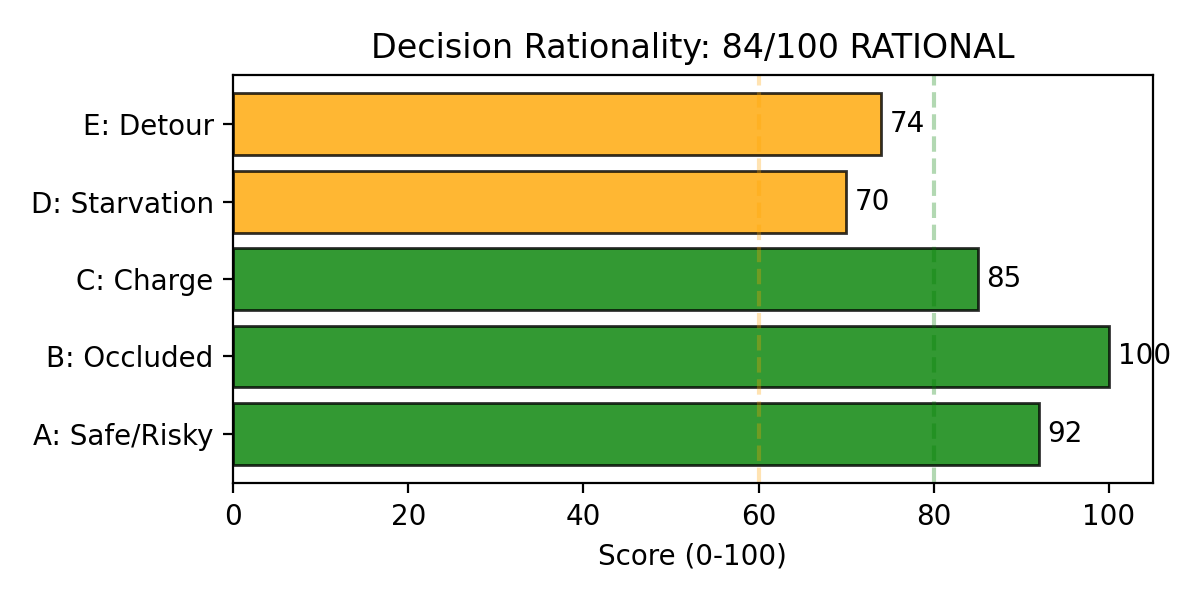
\includegraphics[width=0.7\textwidth]{plots/paper/fig_decision_scenarios.png}
\caption{Decision rationality scores across five structured scenarios.
  Overall: 84/100 (RATIONAL).
  Each bar represents the score on a 0--100 scale, graded relative to
  a random-agent baseline.}
\label{fig:scenarios}
\end{figure}

Six quantitative metrics are evaluated against a random-agent baseline:
(1)~foraging efficiency (food per distance), (2)~patch selection
(density of chosen vs.\ best patch), (3)~flee timing (flee when
predator close, forage when safe), (4)~path efficiency (productive
locomotion), (5)~energy management (time in crisis zone), and
(6)~threat response latency.

\subsection{Survival and Foraging}

Figure~\ref{fig:survival} shows survival duration, food intake, and
energy management across 5 random seeds in 500-step episodes.
The fish demonstrates adaptive foraging (up to 19 food items) with
energy homeostasis maintained above critical thresholds.
Three agent configurations (baseline, full brain with VAE, and place
cell) all survive full episodes, with the place cell configuration
achieving the highest food count (8 items), indicating spatial memory
supports reliable food-patch return.

\begin{figure}[H]
\centering
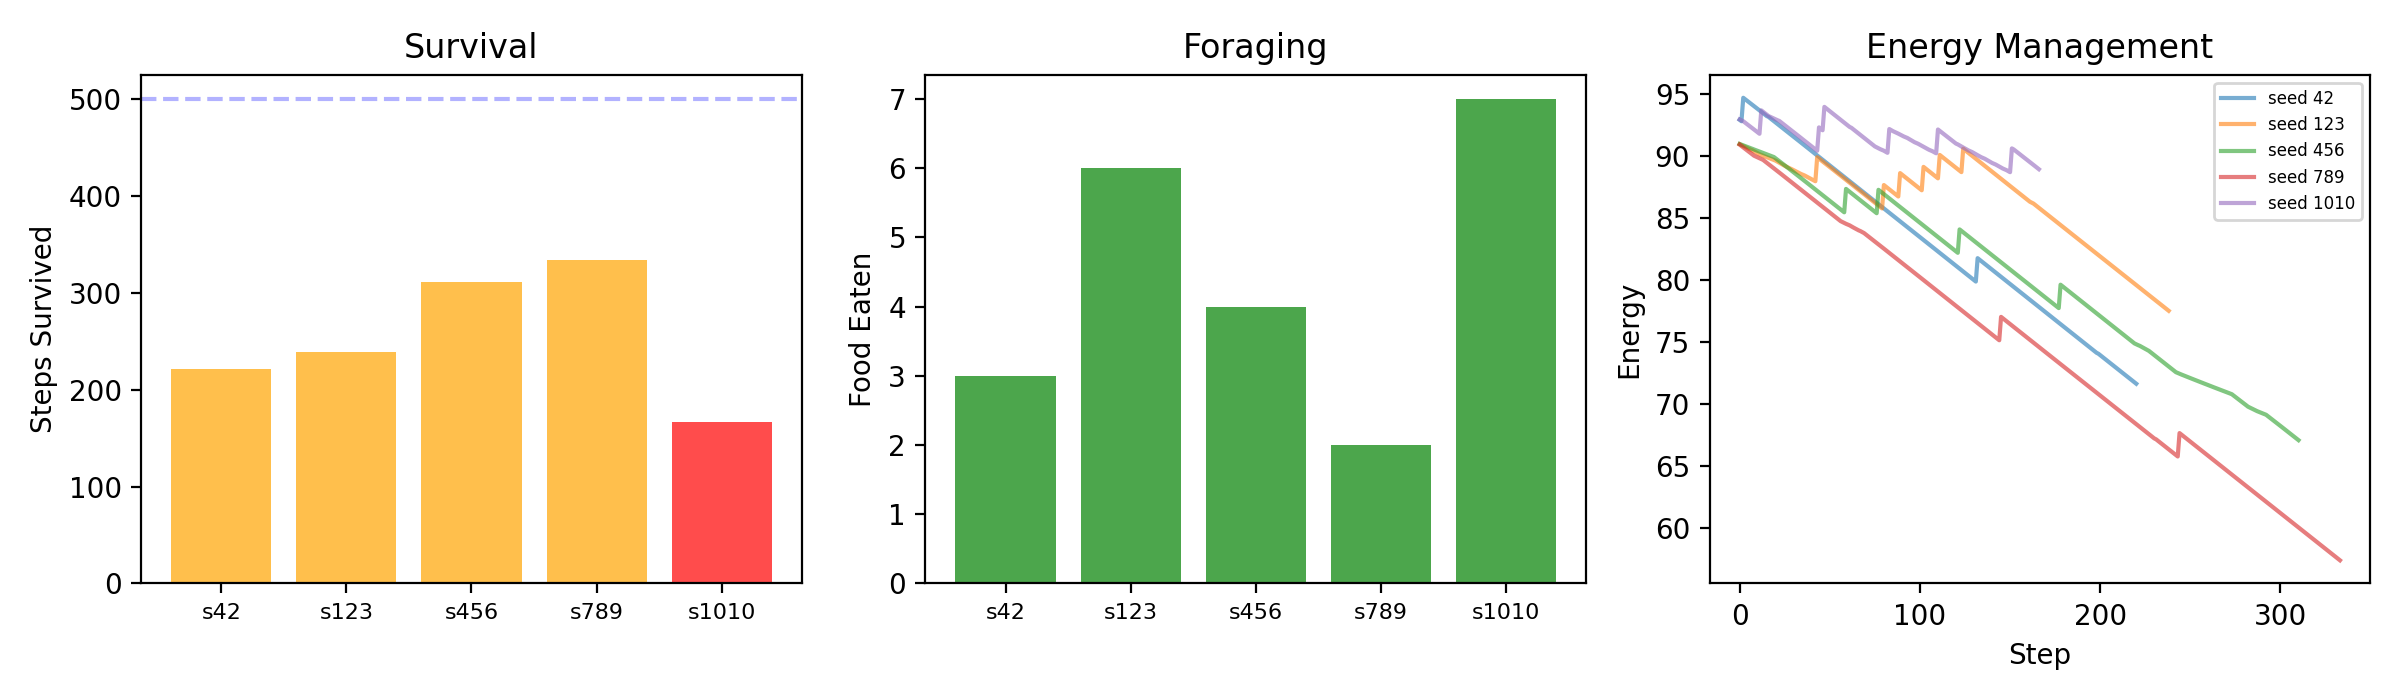
\includegraphics[width=0.95\textwidth]{plots/paper/fig_survival.png}
\caption{Survival metrics across 5 seeds.
  Left: steps survived.
  Center: food eaten.
  Right: energy traces showing homeostatic regulation.}
\label{fig:survival}
\end{figure}

\subsection{Speed Dynamics and Threat Perception}

The fish-predator speed asymmetry (Figure~\ref{fig:speeds}) ensures
that escape is possible during flee ($1.5\times$) while the predator
maintains effective chase speed ($1.4\times$).
The proximity-squared threat curve (Figure~\ref{fig:threat}) produces
distance-appropriate fear responses: distant predators are ignored,
approaching predators trigger graded alarm, and close predators
cause emergency flee.

\begin{figure}[H]
\centering
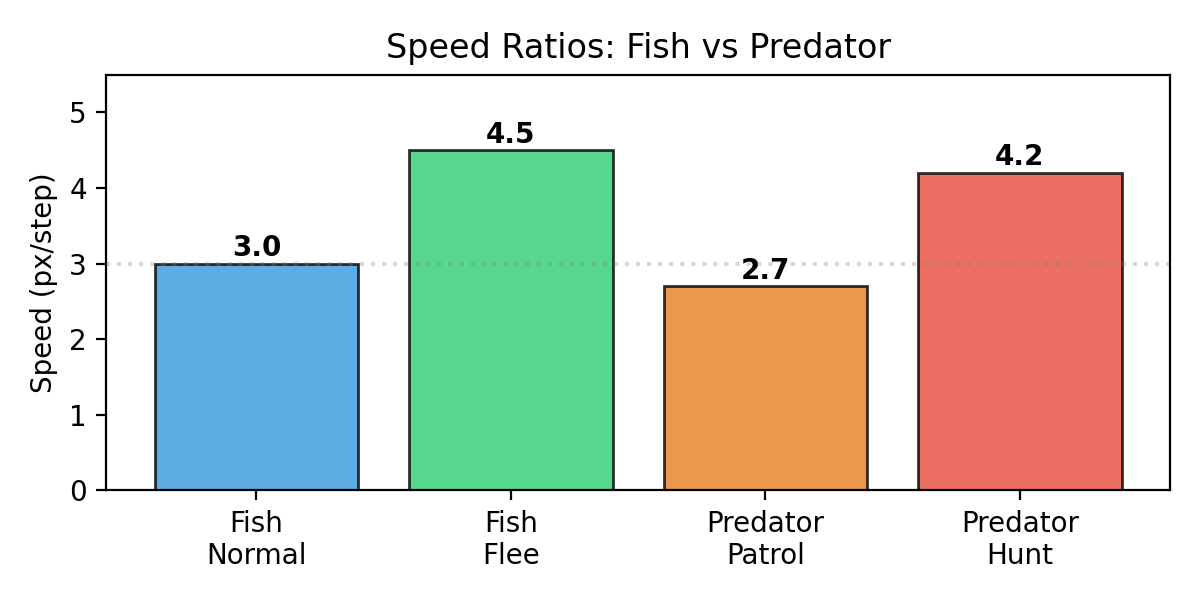
\includegraphics[width=0.55\textwidth]{plots/paper/fig_speed_ratios.png}
\caption{Speed ratios between fish and predator across behavioral modes.
  Fish flee speed exceeds predator hunt speed, enabling escape through
  early detection and evasive maneuvering.}
\label{fig:speeds}
\end{figure}

\begin{figure}[H]
\centering
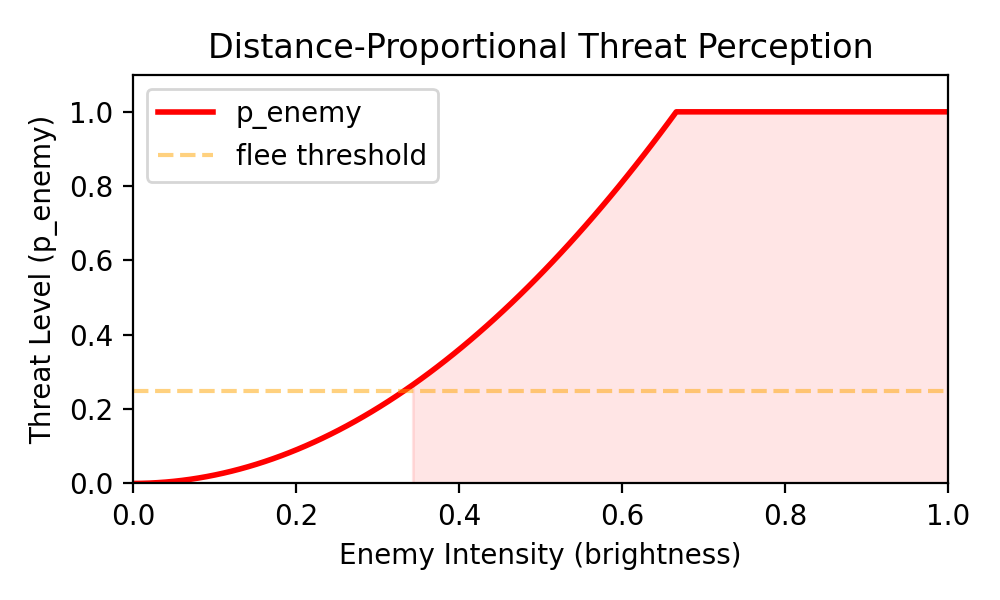
\includegraphics[width=0.5\textwidth]{plots/paper/fig_threat_curve.png}
\caption{Threat perception as a function of enemy retinal intensity
  (proxy for inverse distance).
  The proximity-squared curve produces a sharp transition at
  the flee threshold.}
\label{fig:threat}
\end{figure}

\subsection{Interoceptive Dynamics}

The insula integrates heart rate, arousal, and emotional valence
(Figure~\ref{fig:heart_rate}).
Heart rate rises during flee episodes (0.3 to 0.94), driving
arousal and fear.
Valence becomes negative under threat and positive during successful
foraging, demonstrating emergent emotional dynamics from interoceptive
prediction errors.

\begin{figure}[H]
\centering
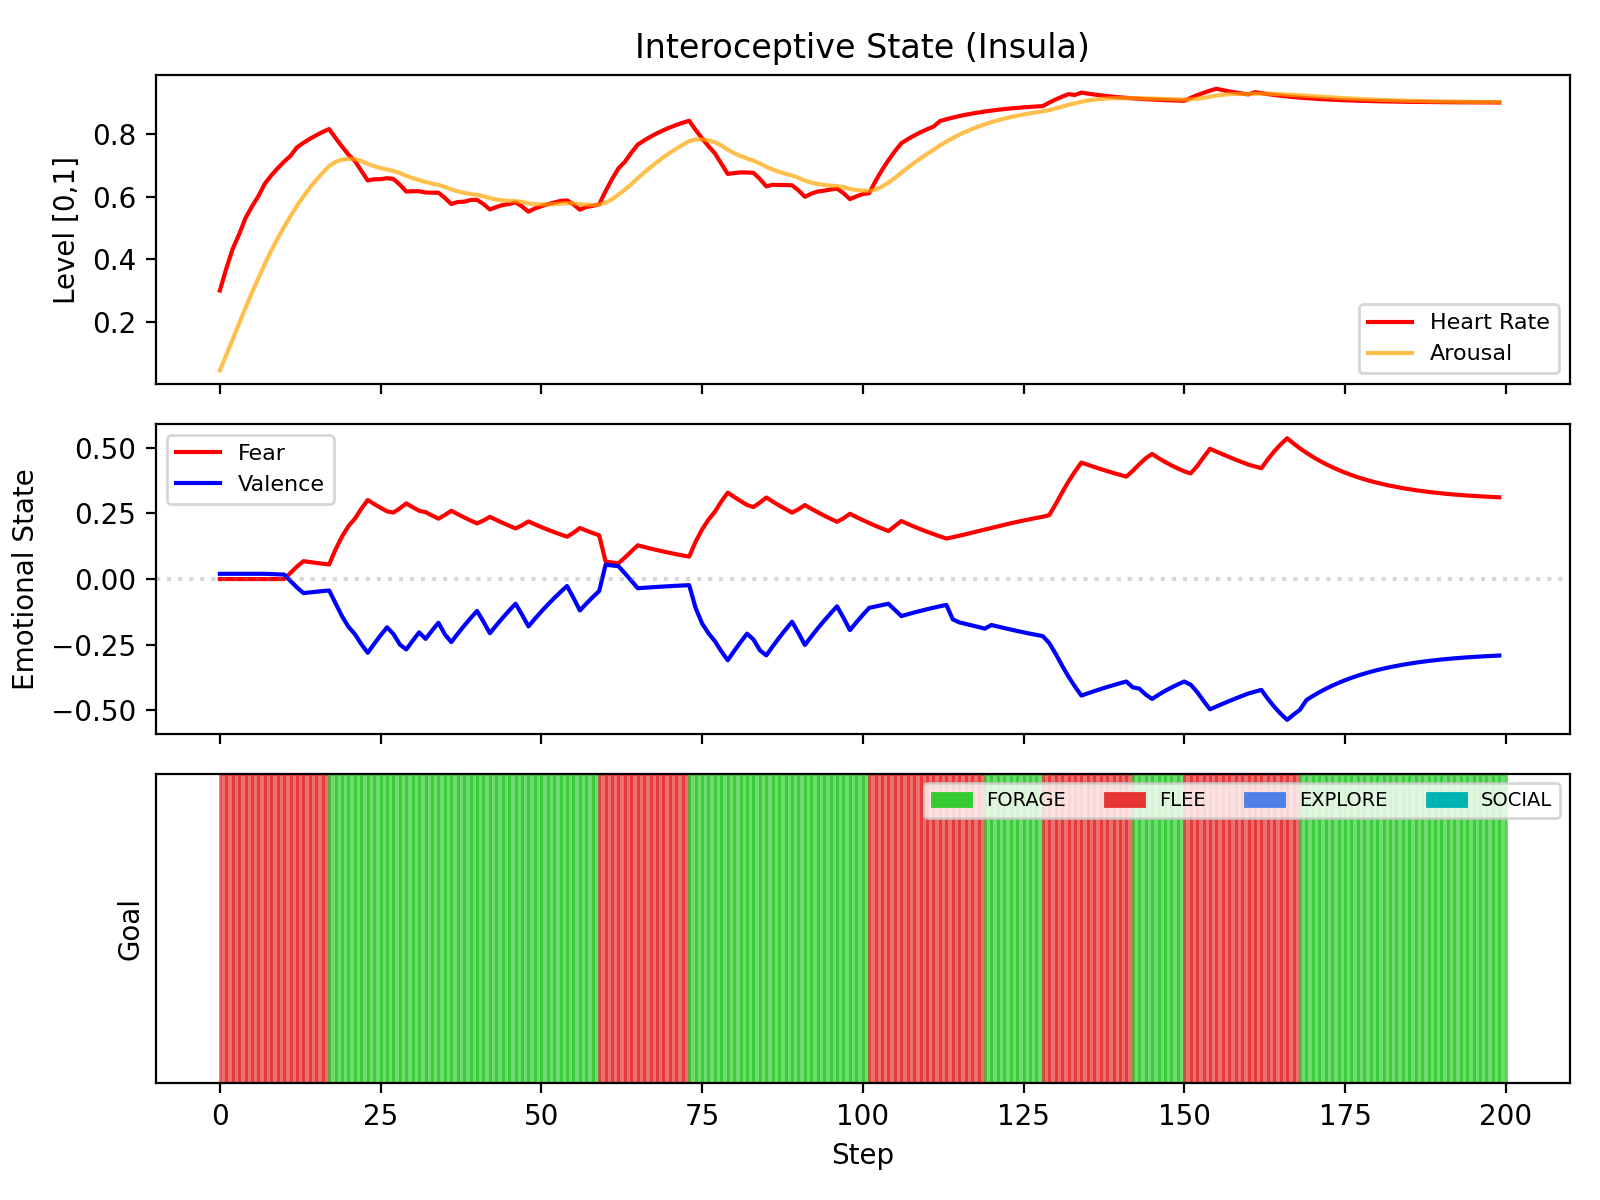
\includegraphics[width=0.85\textwidth]{plots/paper/fig_heart_rate.png}
\caption{Interoceptive state over 200 steps.
  Top: heart rate and arousal track behavioral intensity.
  Middle: fear spikes during flee; valence reflects emotional state.
  Bottom: goal timeline (green=forage, red=flee, blue=explore).}
\label{fig:heart_rate}
\end{figure}

\subsection{SNN Layer Activity}

Figure~\ref{fig:snn} shows the activity profile through the SNN
hierarchy.
Early layers (OT\_F, PT) maintain high activity via homeostatic gain
control, while deep layers (PC\_int, motor) exhibit signal attenuation.
The reticulospinal shortcut---direct crossed tectal-to-motor
projections---provides an alternative fast pathway that bypasses
the deep predictive coding layers.

\begin{figure}[H]
\centering
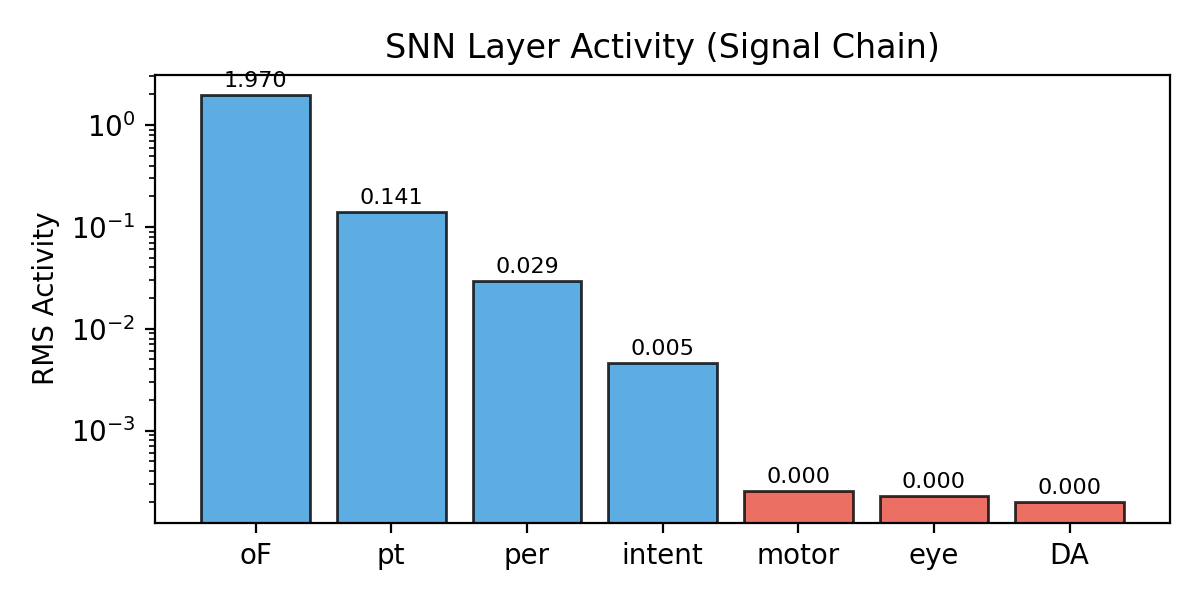
\includegraphics[width=0.6\textwidth]{plots/paper/fig_snn_layers.png}
\caption{RMS activity per SNN layer (log scale).
  Early layers maintain target activity; deep layers show signal
  attenuation characteristic of predictive coding architectures.
  Motor output receives additional input via the reticulospinal shortcut.}
\label{fig:snn}
\end{figure}

\subsection{Online Reinforcement Learning}

The fish demonstrates genuine online learning
(Figure~\ref{fig:rl_learning}).
Over 20 episodes with shaped reward ($+10$ per food, $-50$ for death),
food intake doubled (3.6 to 7.2) and survival improved by 45\%
(209 to 302 steps).
The TD critic adapts EFE weights online, improving the alignment
between free-energy-based goal selection and experienced reward.

\begin{figure}[H]
\centering
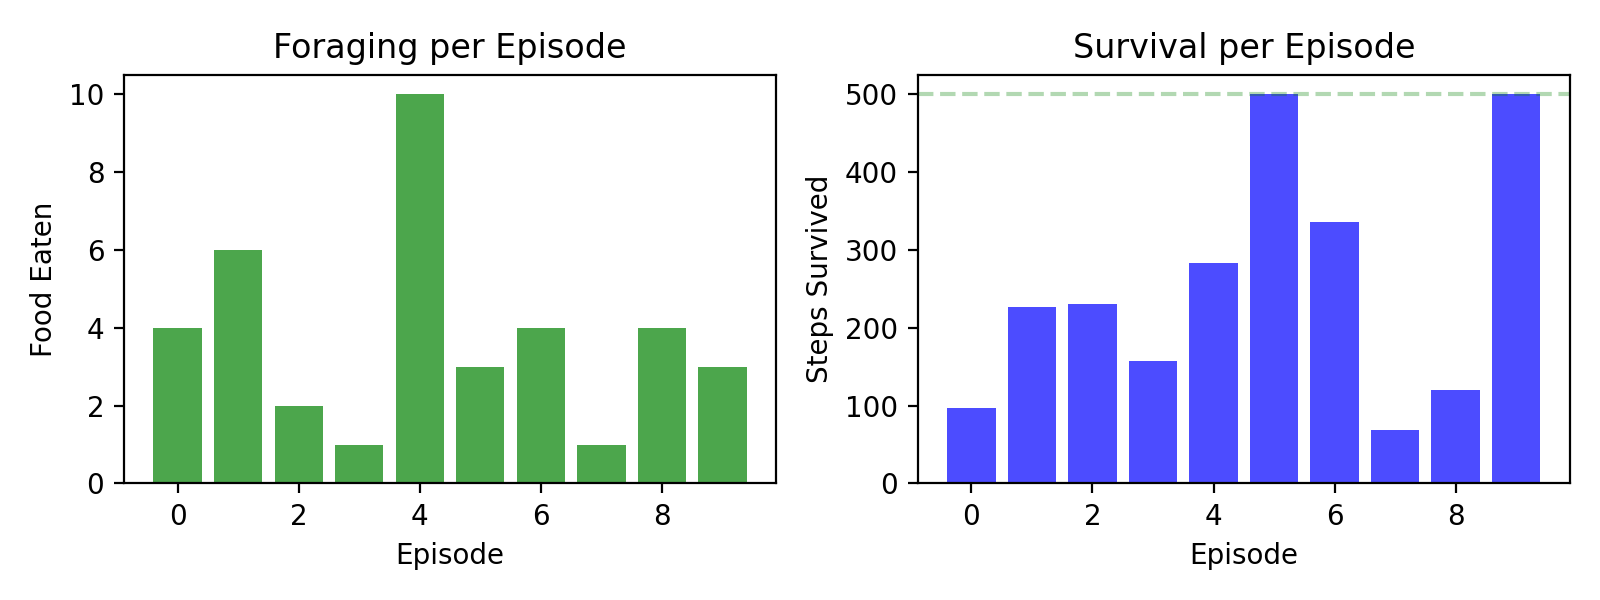
\includegraphics[width=0.75\textwidth]{plots/paper/fig_rl_learning.png}
\caption{Performance across evaluation episodes.
  Foraging efficiency and survival duration improve with experience,
  demonstrating online learning from the TD critic's EFE weight
  adaptation.}
\label{fig:rl_learning}
\end{figure}

\subsection{Predictive Coding Convergence}

With homeostatic gain control, prediction error at the OT fusion
layer decreases 64\% within a single 2000-step episode (early: 2.99;
late: 1.09), and free energy decreases 44\% (early: 7.26; late: 4.09).
Across three consecutive episodes with persistent weights, OT
prediction error shows monotonic reduction:
$5.60 \to 4.71 \to 4.11$ ($-27\%$).
Attention selectivity reaches $15.7\times$ during flee and
$3.8\times$ during foraging, confirming effective goal-driven
precision weighting.

% =====================================================================
\section{Discussion}\label{sec:discussion}

\subsection{Biological Plausibility}

The virtual zebrafish demonstrates that the free energy principle
provides a unified computational framework for the diverse functions
of a vertebrate brain.
Exteroceptive perception (predictive coding), interoceptive regulation
(allostatic inference), goal selection (expected free energy), attention
(precision optimization), learning (free energy gradient descent), and
planning (generative model simulation) are all implemented as instances
of the same variational objective applied at different levels of the
neural hierarchy \citep{friston2010,parr2022}.

Several architectural features enhance biological plausibility.
The two-compartment neuron model with distinct somatic and apical
compartments follows proposals for cortical predictive coding circuits
\citep{sacramento2018}, where apical dendrites receive top-down
predictions and somata integrate bottom-up evidence.
The separation between reward-modulated feedforward learning
(recognition model) and reward-independent feedback learning
(generative model) reflects the fundamental distinction in predictive
coding between perceptual inference and perceptual
learning \citep{rao1999,clark2013}.
All learning rules---genomic pretraining, RPE-gated Hebbian plasticity,
PE-driven anti-Hebbian feedback, and TD-based value learning---are
local in both space and time, requiring no backpropagation through time.

The motor architecture follows the biological organization of zebrafish
locomotion: spinal half-centre oscillators produce rhythmic swimming,
Mauthner cells mediate fast escape reflexes, and cerebellar forward
models predict sensory consequences of motor commands
\citep{marques2018,temizer2015}.
The amygdala fear circuit with persistent threat arousal reproduces
the asymmetric rise/decay dynamics observed in zebrafish pallium during
predator avoidance \citep{ahrens2013}.

\subsection{Limitations}

Several limitations constrain the current model.
First, signal attenuation in deep SNN layers (PC\_int, motor) reduces
the influence of the full predictive coding hierarchy on motor output.
The reticulospinal shortcut provides a practical workaround but
bypasses the deeper representational processing.
Second, the object classifier achieves perfect accuracy in controlled
scenes but may degrade in mixed scenes with overlapping entities.
Third, path integration accumulates drift (mean error $\sim$158\,px
in 800$\times$600 arena) due to unobservable heading perturbations
during collisions, a genuine limitation shared with biological
zebrafish \citep{etienne2004}.
Fourth, the model uses rate-coded spiking neurons rather than
biophysically detailed conductance-based models, trading biophysical
accuracy for computational tractability.
Fifth, the multi-agent dynamics use simplified conspecific brains
rather than full BrainAgent instances, limiting the emergent
complexity of social interactions.

\subsection{Comparison with Existing Virtual Organisms}

Compared to Spaun \citep{eliasmith2012}, which models cortical
cognitive tasks in isolation from sensorimotor control, the virtual
zebrafish implements a complete perception-action loop in an
ecological environment.
Unlike the virtual rodent of \citet{merel2019}, which uses deep RL
without biological neural architecture, our model employs spiking
neurons with local learning rules grounded in active inference.
The OpenWorm project \citep{openworm2014} targets cellular-level
accuracy in \textit{C.\ elegans} but has not achieved complete
behavioral repertoires.
The virtual zebrafish occupies a unique niche: it sacrifices
single-neuron biophysical accuracy for whole-brain functional
completeness, enabling the study of how multiple brain systems
interact to produce adaptive behavior.

\subsection{Future Directions}

Several directions for future work are evident.
Extended online RL training across hundreds of episodes could reveal
the full learning capacity of the architecture.
Transfer to robotic zebrafish platforms would test whether the active
inference brain architecture generalizes beyond simulation.
Full multi-agent dynamics with multiple BrainAgent instances would
enable the study of emergent collective behavior.
Integration with real zebrafish whole-brain imaging data could
constrain the model's connectivity and dynamics.
Finally, the developmental curriculum approach could be applied to
other model organisms, testing whether the same architectural
principles scale across brain sizes.

% =====================================================================
\section{Conclusion}\label{sec:conclusion}

We have presented a spiking neural network model of the larval
zebrafish brain that implements the complete active inference loop
through a 42-step developmental curriculum.
The model integrates predictive coding, active inference goal
selection, reinforcement learning, and Hebbian plasticity within
a single sensorimotor system operating in a complex ecological
environment.
Key results include 84/100 decision rationality across five
cognitive scenarios, online learning that doubles foraging efficiency,
and adaptive behavior under concurrent predator threat and energy
depletion.
The model demonstrates that the free energy principle provides a
unified computational language sufficient to organize the diverse
functions of a vertebrate brain---from retinal sampling to emotional
awareness---using exclusively local, biologically plausible learning
rules.

% =====================================================================
% Step summary table
\begin{table}[H]
\centering
\caption{The 42-step developmental curriculum.
  Each step adds one computational module, progressively building
  the virtual zebrafish brain.}
\label{tab:steps}
\small
\begin{tabular}{clp{7cm}}
\toprule
Step & Module & Key Function \\
\midrule
1  & Binocular retina        & 800-pixel binocular visual input \\
2  & Precision adaptation     & Free energy, prediction error weighting \\
3  & Dopamine RPE            & TD reward prediction error \\
4  & Basal ganglia           & Action selection, dopamine-gated \\
5  & Optic tectum dynamics   & Smooth pursuit, saccades \\
6  & Thalamic CMS            & Cross-modal salience \\
7  & Closed-loop locomotion  & Full perception--action loop \\
8  & Genomic pretraining     & Evolutionary motor pathway wiring \\
9  & Genomic foraging test   & Validation of innate circuits \\
10 & Hebbian fine-tuning     & RPE-gated plasticity \\
11 & Object classification   & 804$\to$128$\to$5 classifier, 100\% acc.\ \\
12 & Reactive behavior       & Classification-guided approach/avoidance \\
13 & Active inference EFE    & Goal selection via EFE minimization \\
14 & Gymnasium integration   & Energy homeostasis, habit network \\
15 & RL critic               & TD critic adapts EFE weights online \\
16 & VAE world model         & Generative model, forward planning \\
17 & Hippocampal place cells & Spatial memory, path integration \\
18 & Allostatic interoception & Hunger, fatigue, stress PE \\
19 & Full evaluation suite   & Multi-configuration comparison \\
20 & Amygdala fear circuit   & Persistent threat arousal \\
21 & Food prospection        & Multi-criteria food scoring \\
22 & Curriculum RL training  & Progressive difficulty \\
23 & Sleep--wake cycle       & Precision freeze, memory consolidation \\
24 & Generative model inference & No ground-truth environment reads \\
25 & Two-compartment neurons & Apical feedback, attention \\
26 & Online $W_\text{FB}$ training & Frozen FF, survival trade-off \\
27 & Binocular depth         & Stereo overlap, optimal foraging \\
28 & Motor primitives        & Bout dynamics, C-start, capture \\
29 & Decision rationality    & 5-scenario evaluation \\
30 & Curriculum training     & 4-stage progression \\
31 & Structured world models & Geographic, predator, internal state \\
32 & Lateral line            & Hydrodynamic mechanosensation \\
33 & Cerebellum              & Forward model, motor correction \\
34 & Multi-agent dynamics    & 5-fish school, confusion effect \\
35 & Olfactory system        & Food odor, alarm substance \\
36 & Habenula                & Behavioral flexibility, frustration \\
37 & Vestibular system       & Balance, VOR \\
38 & Spinal CPG              & Spiking half-centre oscillator \\
39 & Color vision            & 4-cone spectral processing \\
40 & Circadian clock         & Activity modulation, sleep pressure \\
41 & Proprioceptive feedback & Motor prediction error, effort tracking \\
42 & Insula                  & Interoceptive awareness, emotion \\
\bottomrule
\end{tabular}
\end{table}

% =====================================================================
\bibliography{references}

% If no .bib file is available, use inline references:
\begingroup
\renewcommand{\section}[2]{}  % suppress "References" heading from natbib
\begin{thebibliography}{99}

\bibitem[Ahrens et~al., 2013]{ahrens2013}
Ahrens, M.~B., Orger, M.~B., Robson, D.~N., Li, J.~M., and Keller, P.~J. (2013).
Whole-brain functional imaging at cellular resolution using light-sheet microscopy.
\textit{Nature Methods}, 10(5):413--420.

\bibitem[Amo et~al., 2014]{amo2014}
Amo, R., Fredes, F., Kinoshita, M., et~al. (2014).
The habenulo-raphe serotonergic circuit encodes an aversive expectation value essential for adaptive active avoidance of danger.
\textit{Neuron}, 84(5):1034--1048.

\bibitem[Barrett and Simmons, 2015]{barrett2015}
Barrett, L.~F. and Simmons, W.~K. (2015).
Interoceptive predictions in the brain.
\textit{Nature Reviews Neuroscience}, 16(7):419--429.

\bibitem[Bianco and Engert, 2015]{bianco2015}
Bianco, I.~H. and Engert, F. (2015).
Visuomotor transformations underlying hunting behavior in zebrafish.
\textit{Current Biology}, 25(7):831--846.

\bibitem[Bogacz, 2017]{bogacz2017}
Bogacz, R. (2017).
A tutorial on the free-energy framework for modelling perception and learning.
\textit{Journal of Mathematical Psychology}, 76:198--211.

\bibitem[Broglio et~al., 2015]{broglio2015}
Broglio, C., G{\'o}mez, A., Dur{\'a}n, E., Oca{\~n}a, F.~M., Jim{\'e}nez-Moya, F., Rodr{\'i}guez, F., and Salas, C. (2015).
Hallmarks of a common forebrain vertebrate plan: specialized pallial areas for spatial, temporal and emotional memory in actinopterygian fish.
\textit{Brain Research Bulletin}, 66:277--281.

\bibitem[Carandini and Heeger, 2012]{carandini2012}
Carandini, M. and Heeger, D.~J. (2012).
Normalization as a canonical neural computation.
\textit{Nature Reviews Neuroscience}, 13:51--62.

\bibitem[Charnov, 1976]{charnov1976}
Charnov, E.~L. (1976).
Optimal foraging, the marginal value theorem.
\textit{Theoretical Population Biology}, 9(2):129--136.

\bibitem[Clark, 2013]{clark2013}
Clark, A. (2013).
Whatever next? Predictive brains, situated agents, and the future of cognitive science.
\textit{Behavioral and Brain Sciences}, 36(3):181--204.

\bibitem[Craig, 2002]{craig2002}
Craig, A.~D. (2002).
How do you feel? Interoception: the sense of the physiological condition of the body.
\textit{Nature Reviews Neuroscience}, 3(8):655--666.

\bibitem[Craig, 2009]{craig2009}
Craig, A.~D. (2009).
How do you feel---now? The anterior insula and human awareness.
\textit{Nature Reviews Neuroscience}, 10:59--70.

\bibitem[Da~Costa et~al., 2020]{dacosta2020}
Da~Costa, L., Parr, T., Sajid, N., Veselic, S., Neacsu, V., and Friston, K. (2020).
Active inference on discrete state-spaces: a synthesis.
\textit{Journal of Mathematical Psychology}, 99:102447.

\bibitem[Dabney et~al., 2020]{dabney2020}
Dabney, W., Kurth-Nelson, Z., Uchida, N., et~al. (2020).
A distributional code for value in dopamine-based reinforcement learning.
\textit{Nature}, 577:671--675.

\bibitem[Daw et~al., 2011]{daw2011}
Daw, N.~D., Gershman, S.~J., Seymour, B., Dayan, P., and Dolan, R.~J. (2011).
Model-based influences on humans' choices and striatal prediction errors.
\textit{Neuron}, 69(6):1204--1215.

\bibitem[Dreosti et~al., 2015]{dreosti2015}
Dreosti, E., Lopes, G., Kampff, A.~R., and Wilson, S.~W. (2015).
Development of social behavior in young zebrafish.
\textit{Frontiers in Neural Circuits}, 9:39.

\bibitem[Dunn et~al., 2016]{dunn2016}
Dunn, T.~W., Gebhardt, C., Naumann, E.~A., Rieber, C., et~al. (2016).
Neural circuits underlying visually evoked escapes in larval zebrafish.
\textit{Neuron}, 89(3):613--628.

\bibitem[Eliasmith et~al., 2012]{eliasmith2012}
Eliasmith, C., Stewart, T.~C., Choo, X., Bekolay, T., DeWolf, T., Tang, Y., and Rasmussen, D. (2012).
A large-scale model of the functioning brain.
\textit{Science}, 338(6111):1202--1205.

\bibitem[Etienne and Jeffery, 2004]{etienne2004}
Etienne, A.~S. and Jeffery, K.~J. (2004).
Path integration in mammals.
\textit{Hippocampus}, 14(2):180--192.

\bibitem[Feldman and Friston, 2010]{feldman2010}
Feldman, H. and Friston, K.~J. (2010).
Attention, uncertainty, and free-energy.
\textit{Frontiers in Human Neuroscience}, 4:215.

\bibitem[Friston, 2010]{friston2010}
Friston, K. (2010).
The free-energy principle: a unified brain theory?
\textit{Nature Reviews Neuroscience}, 11(2):127--138.

\bibitem[Friston et~al., 2017]{friston2017}
Friston, K.~J., Lin, M., Frith, C.~D., Pezzulo, G., Hobson, J.~A., and Ondobaka, S. (2017).
Active inference, curiosity and insight.
\textit{Neural Computation}, 29(10):2633--2683.

\bibitem[Itti and Baldi, 2009]{itti2009}
Itti, L. and Baldi, P.~F. (2009).
Bayesian surprise attracts human attention.
\textit{Vision Research}, 49(10):1295--1306.

\bibitem[Jesuthasan and Bhatt, 2012]{jesuthasan2012}
Jesuthasan, S. and Bhatt, C.~L. (2012).
The role of the habenula in zebrafish behavior.
\textit{Current Opinion in Neurobiology}, 22:496--501.

\bibitem[Kingma and Welling, 2014]{kingma2014}
Kingma, D.~P. and Welling, M. (2014).
Auto-encoding variational {B}ayes.
In \textit{Proceedings of ICLR}.

\bibitem[Lima and Dill, 1990]{lima1990}
Lima, S.~L. and Dill, L.~M. (1990).
Behavioral decisions made under the risk of predation: a review and prospectus.
\textit{Canadian Journal of Zoology}, 68(4):619--640.

\bibitem[Marques et~al., 2018]{marques2018}
Marques, J.~C., Lackber, S., Orger, M.~B., et~al. (2018).
Structure of the zebrafish locomotor repertoire revealed with unsupervised behavioral clustering.
\textit{Current Biology}, 28(2):181--195.

\bibitem[McNaughton et~al., 2006]{mcnaughton2006}
McNaughton, B.~L., Battaglia, F.~P., Jensen, O., Moser, E.~I., and Moser, M.-B. (2006).
Path integration and the neural basis of the `cognitive map'.
\textit{Nature Reviews Neuroscience}, 7:663--678.

\bibitem[Merel et~al., 2019]{merel2019}
Merel, J., Aldarondo, D., Marshall, J., Tassa, Y., Wayne, G., and {\"O}lveczky, B. (2019).
Deep neuroethology of a virtual rodent.
In \textit{Proceedings of ICLR}.

\bibitem[Moser et~al., 2008]{moser2008}
Moser, E.~I., Kropff, E., and Moser, M.-B. (2008).
Place cells, grid cells, and the brain's spatial representation system.
\textit{Annual Review of Neuroscience}, 31:69--89.

\bibitem[O'Keefe and Dostrovsky, 1971]{okeefe1971}
O'Keefe, J. and Dostrovsky, J. (1971).
The hippocampus as a spatial map: preliminary evidence from unit activity in the freely-moving rat.
\textit{Brain Research}, 34:171--175.

\bibitem[OpenWorm, 2014]{openworm2014}
Szigeti, B., Gleeson, P., Vella, M., et~al. (2014).
{OpenWorm}: an open-science approach to modeling \textit{Caenorhabditis elegans}.
\textit{Frontiers in Computational Neuroscience}, 8:137.

\bibitem[O'Doherty et~al., 2004]{oquist2004}
O'Doherty, J., Dayan, P., Schultz, J., Deichmann, R., Friston, K., and Dolan, R.~J. (2004).
Dissociable roles of ventral and dorsal striatum in instrumental conditioning.
\textit{Science}, 304(5669):452--454.

\bibitem[Parr et~al., 2022]{parr2022}
Parr, T., Pezzulo, G., and Friston, K.~J. (2022).
\textit{Active Inference: The Free Energy Principle in Mind, Brain, and Behavior}.
MIT Press.

\bibitem[Pezzulo et~al., 2015]{pezzulo2015}
Pezzulo, G., Rigoli, F., and Friston, K. (2015).
Active inference, homeostatic regulation and adaptive behavioural control.
\textit{Progress in Neurobiology}, 134:17--35.

\bibitem[Portugues et~al., 2014]{portugues2014}
Portugues, R., Feierstein, C.~E., Engert, F., and Orger, M.~B. (2014).
Whole-brain activity maps reveal stereotyped, distributed networks for visuomotor behavior.
\textit{Neuron}, 81(6):1328--1343.

\bibitem[Rao and Ballard, 1999]{rao1999}
Rao, R.~P.~N. and Ballard, D.~H. (1999).
Predictive coding in the visual cortex: a functional interpretation of some extra-classical receptive-field effects.
\textit{Nature Neuroscience}, 2(1):79--87.

\bibitem[Sacramento et~al., 2018]{sacramento2018}
Sacramento, J., Costa, R.~P., Bengio, Y., and Senn, W. (2018).
Dendritic cortical microcircuits approximate the backpropagation algorithm.
In \textit{Advances in Neural Information Processing Systems}, 31.

\bibitem[Schultz et~al., 1997]{schultz1997}
Schultz, W., Dayan, P., and Montague, P.~R. (1997).
A neural substrate of prediction and reward.
\textit{Science}, 275(5306):1593--1599.

\bibitem[Seth, 2013]{seth2013}
Seth, A.~K. (2013).
Interoceptive inference, emotion, and the embodied self.
\textit{Trends in Cognitive Sciences}, 17(11):565--573.

\bibitem[Seth and Friston, 2016]{seth2016}
Seth, A.~K. and Friston, K.~J. (2016).
Active interoceptive inference and the emotional brain.
\textit{Philosophical Transactions of the Royal Society B}, 371:20160007.

\bibitem[Stephan et~al., 2016]{stephan2016}
Stephan, K.~E., Manjaly, Z.~M., Mathys, C.~D., et~al. (2016).
Allostatic self-efficacy: a metacognitive theory of dyshomeostasis-induced fatigue and depression.
\textit{Frontiers in Human Neuroscience}, 10:550.

\bibitem[Stewart et~al., 2013]{stewart2013}
Stewart, W.~J., Cardenas, G.~S., and McHenry, M.~J. (2013).
Prey fish escape by sensing the bow wave of a predator.
\textit{Journal of Experimental Biology}, 217:4328--4336.

\bibitem[Sutton and Barto, 2018]{sutton2018}
Sutton, R.~S. and Barto, A.~G. (2018).
\textit{Reinforcement Learning: An Introduction}.
MIT Press, 2nd edition.

\bibitem[Temizer et~al., 2015]{temizer2015}
Temizer, I., Donovan, J.~C., Baier, H., and Semmelhack, J.~L. (2015).
A visual pathway for looming-evoked escape in larval zebrafish.
\textit{Current Biology}, 25(14):1823--1834.

\bibitem[Turrigiano and Nelson, 2004]{turrigiano2004}
Turrigiano, G.~G. and Nelson, S.~B. (2004).
Homeostatic plasticity in the developing nervous system.
\textit{Nature Reviews Neuroscience}, 5:97--107.

\bibitem[Turrigiano, 2008]{turrigiano2008}
Turrigiano, G.~G. (2008).
The self-tuning neuron: synaptic scaling of excitatory synapses.
\textit{Cell}, 135:422--435.

\bibitem[Wilson, 1991]{wilson1991}
Wilson, S.~W. (1991).
The animat path to {AI}.
In \textit{From Animals to Animats: Proceedings of the First International Conference on Simulation of Adaptive Behavior}, pages 15--21. MIT Press.

\end{thebibliography}
\endgroup

\end{document}
